% Provenance (never printed): see sources/outline_sources.md (Year 1: continental
% rifting and break-up; passive-margin structure; fast and slow ridges; the depth--age
% law of the ocean floor; transform faults). Curve from figdata/bachelor-1/depth_age.py;
% exercise and problem values in the Book 3 scratch calculator calc/ch13.py; the
% coordinates of the margin schematic from calc/fig13_margin.py.
\chapter{Rifts, dorsales et marges passives}\label{ch:b1:rifts-ridges-margins}

En septembre 2005, le sol du désert de l'Afar, dans le nord-est de l'Éthiopie,
s'est ouvert. En trois semaines un tronçon de rift long d'environ \qty{60}{km} s'est élargi de
jusqu'à \qty{8}{m}, et environ \qty{2.5}{km^3} de magma sont montés dans la fissure depuis
le dessous. Les plaques s'y écartent d'environ \qty{18}{mm} par an~: la crise
a libéré, en quelques semaines, l'étirement d'environ quatre siècles. L'Afar est un
continent qui se brise~; quelques centaines de kilomètres plus au nord, la mer Rouge
est un jeune océan dont le plancher est déjà fait comme celui de l'Atlantique,
et l'Atlantique sud était un tel rift avant de s'ouvrir, il y a environ 120 millions
d'années. Ce chapitre suit la naissance d'un océan~: l'étirement d'un
continent, sa rupture, les deux \omterm{def:b1:rifts-ridges-margins:passive-margin}{marges passives} laissées derrière,
la dorsale qui construit le plancher océanique, et l'enfoncement lent de ce plancher à mesure qu'il se refroidit.
% ledger: wright:afar, morvel:ar-nb (18.5 mm/yr at 12.3 N, 40.6 E, computed with euler_velocities.py), heine:fit

\begin{recall}
Les plaques sont la \omterm{def:b1:heat-budget:boundary-layer}{couche limite thermique} supérieure du \omterm{def:b1:layered-earth:layers}{manteau}~; sous les
océans un demi-espace en refroidissement les décrit, et leurs isothermes s'approfondissent comme la
racine carrée de l'âge (\cref{ch:b1:heat-budget}). Des colonnes de roche en équilibre
isostatique ont la même masse par unité d'aire au-dessus d'une \omterm{def:b1:isostasy-gravity:isostasy}{profondeur de compensation}
(\cref{ch:b1:isostasy-gravity}). Les plaques tournent autour de \omterm{def:b1:plate-kinematics:euler-pole}{pôles d'Euler}, les dorsales s'ouvrent
à des vitesses lues sur les anomalies magnétiques, et les transformantes se placent sur des \omterm{def:b1:spherical-astronomy:spherical-triangle}{petits cercles}
autour du pôle (\cref{ch:b1:plate-kinematics}). Le \omterm{def:b1:cross-sections:throw}{rejet vertical} et le \omterm{def:b1:cross-sections:throw}{rejet horizontal} d'une
faille ont été définis au \cref{ch:b1:cross-sections}~; une faille normale est une faille
inclinée dont le compartiment supérieur s'est abaissé (livre~2, année~11).
\end{recall}

\section{Le rifting continental}

Un continent étiré par des forces à ses bords ne s'amincit pas uniformément. Sa \omterm{def:b1:layered-earth:layers}{croûte}
supérieure cassante se brise le long de failles normales, et les blocs entre elles s'enfoncent
et basculent~; en dessous, la \omterm{def:b1:layered-earth:layers}{croûte} inférieure plus chaude et le \omterm{def:b1:layered-earth:layers}{manteau} s'écoulent.

\begin{definition}[Rift continental, graben, demi-graben]\label{def:b1:rifts-ridges-margins:rift}
Un \emph{rift continental}\index{rift continental} est une zone longue et étroite où
un continent est étiré~: une dépression bordée de failles normales, avec
des séismes et, souvent, des volcans. Un \emph{graben}\index{graben} est un bloc
affaissé entre deux failles normales qui plongent l'une vers l'autre. Un
\emph{demi-graben}\index{demi-graben} est un bloc affaissé et basculé contre une
seule faille normale majeure, la faille bordière, d'un seul côté.
\end{definition}

La plupart des bassins de rift sont des chaînes de \omterm{def:b1:rifts-ridges-margins:rift}{demi-grabens}. Leurs failles bordières se
passent le déplacement par des rampes de relais, et le côté de la
faille bordière alterne souvent d'un segment au suivant. Le toit
de chaque faille bordière bascule vers elle, et le bassin se remplit le plus vite là~:
les sédiments les plus épais s'accumulent contre la faille, tandis que le mur est soulevé
en épaulement du rift.

L'étirement horizontal porté par une faille est son \omterm{def:b1:cross-sections:throw}{rejet horizontal}. Une faille normale
plane de \omterm{def:b1:cross-sections:throw}{rejet vertical} $h$ et de \omterm{def:b1:geological-maps:attitude}{pendage} $\delta$ a pour \omterm{def:b1:cross-sections:throw}{rejet horizontal} $h/\tan\delta$
(\cref{ch:b1:cross-sections})~; en additionnant les rejets horizontaux des failles d'une
coupe de rift on obtient l'extension de la \omterm{def:b1:layered-earth:layers}{croûte} cassante. Comment toute la \omterm{def:b1:layered-earth:lithosphere}{lithosphère}
s'amincit quand elle est étirée, et pourquoi elle s'enfonce ensuite, est quantifié dans le volume
de deuxième année~; ici les failles sont mesurées, et leur somme comparée au mouvement
des plaques.

\begin{omfigure}
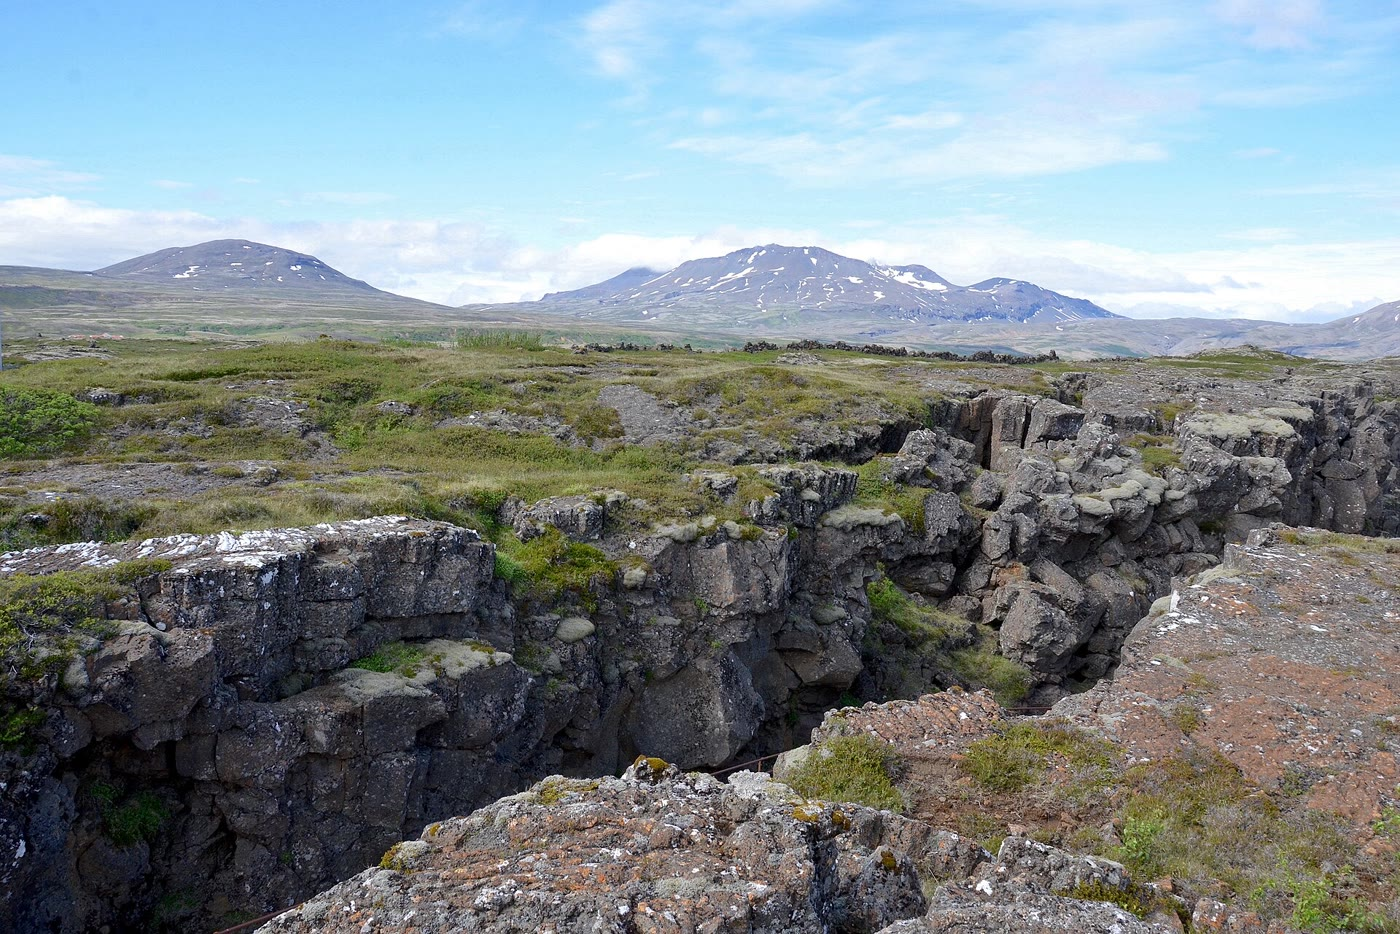
\includegraphics[width=0.8\linewidth]{images/book3/b1-thingvellir-fissure.jpg}

\par\smallskip{\small Une fissure ouverte dans le plancher de lave de la vallée du rift de
Þingvellir, dans le sud-ouest de l'Islande, où la dorsale médio-atlantique émerge.
Les coulées de basalte du fond de la vallée sont coupées par des fissures ouvertes parallèles au
rift. Photographie~: Olga Ernst,
CC~BY-SA~4.0 (Wikimedia Commons).}
\label{fig:b1:rifts-ridges-margins:thingvellir}
\end{omfigure}
% ledger: commons:thingvellir

\subsection*{Rifts volcaniques et rifts pauvres en magma}

Les rifts diffèrent par la quantité de magma qu'ils reçoivent. Dans un rift \emph{pauvre en magma}
l'étirement est repris par des failles, et la \omterm{def:b1:layered-earth:layers}{croûte} s'amincit à mesure que les blocs glissent
l'un de l'autre. Dans un rift volcanique le magma prend le relais~: des dykes recoupent la \omterm{def:b1:layered-earth:layers}{croûte} le long de
l'axe, chacun ouvrant le rift de sa propre épaisseur, et des laves inondent la
surface. Le rift est-africain montre les deux, côte à côte~: sa branche orientale
est fortement volcanique, tandis que sa branche occidentale l'est moins et contient de profonds
bassins sédimentaires, remplis par des lacs comme le lac Tanganyika et bordés de
failles.
% ledger: roberts:ear

Les deux branches ont commencé à se former il y a environ 25 millions d'années, et le rift divise
la plaque africaine en une plaque nubienne à l'ouest et une plaque somalienne à
l'est. Du \omterm{def:b1:plate-kinematics:triple-junction}{point triple} de l'Afar il court vers le sud, en deux branches autour du
vieux craton de Tanzanie, épais et froid. Son mouvement est lent~: calculée
à partir des vecteurs de plaques de la Somalie et de la Nubie, chacun mesuré par rapport à la
plaque antarctique, la Somalie s'éloigne de la Nubie à \qty{6.0}{mm.an^{-1}}
vers \ang{105} dans l'Éthiopie centrale (\ang{8.5}\,N, \ang{39.5}\,E), et à
\qty{5.1}{mm.an^{-1}} sur l'équateur. De nombreux séismes du rift montrent une
faille normale.
% ledger: roberts:ear, morvel:sm-an, morvel:nb-an (SM-NB from SM-AN minus NB-AN, computed with figdata/bachelor-1/euler_velocities.py)

En Afar, à l'extrémité nord, le rift rencontre la mer Rouge et le golfe d'Aden.
L'essentiel des basaltes de trapps éthiopiens y a été émis il y a environ 30 millions d'années,
en un million d'années ou moins, et le magma n'a cessé d'arriver depuis~: coulées
en surface, intrusions dans la \omterm{def:b1:layered-earth:layers}{croûte} et matériau nouveau ajouté en dessous, tant
que la \omterm{def:b1:layered-earth:layers}{croûte} intrudée a gardé son épaisseur pendant les premiers stades
du rifting. La crise de 2005 montre comment un tel rift s'ouvre~: pas régulièrement, mais
par épisodes, chacun un dyke large de quelques mètres injecté en quelques jours ou semaines. Comme les
plaques divergent d'environ \qty{18}{mm.an^{-1}} là, le dyke de \qty{8}{m} de
2005 a repris l'étirement d'environ 440 ans.
% ledger: hofmann:traps, bastow:afar, wright:afar, morvel:ar-nb (rate computed with euler_velocities.py)

\section{Rupture continentale et marges passives}

Si l'étirement continue, la \omterm{def:b1:layered-earth:layers}{croûte} continentale s'amincit jusqu'à disparaître, le \omterm{def:b1:layered-earth:layers}{manteau}
monte sous le rift et fond en montant, et la première \omterm{def:b1:rifts-ridges-margins:oceanic-crust}{croûte océanique}
se forme entre les deux moitiés du continent. Ce moment est la
\emph{rupture continentale}. À partir de là les plaques s'écartent à une dorsale au milieu
d'un nouvel océan, et les deux bords du continent, éloignés de la dorsale,
cessent d'être des limites de plaques.

\begin{definition}[Marge passive, transition océan--continent, discordance de rupture]\label{def:b1:rifts-ridges-margins:passive-margin}
Une \emph{marge passive}\index{marge passive} est le bord d'un continent qui
s'est formé par rifting et n'est plus une limite de plaques~: le continent et le
plancher océanique adjacent appartiennent à la même plaque. La
\emph{transition océan--continent}\index{transition ocean--continent@transition océan--continent} est la
zone de la marge, large de kilomètres à dizaines de kilomètres, entre la \omterm{def:b1:layered-earth:layers}{croûte}
continentale amincie et la \omterm{def:b1:rifts-ridges-margins:oceanic-crust}{croûte océanique} normale. La \emph{discordance de
rupture}\index{discordance de rupture} est la \omterm{def:b1:cross-sections:unconformity}{discordance} qui sépare
les sédiments déposés dans les bassins de rift, basculés avec leurs blocs, des
sédiments non perturbés déposés sur la marge après la rupture.
\end{definition}

Les \omterm{def:b1:rifts-ridges-margins:passive-margin}{marges passives} bordent l'essentiel de l'Atlantique, de l'océan Arctique et de l'ouest de l'océan
Indien, et presque toutes les côtes de l'Afrique, de l'Australie, du Groenland et de l'Inde. La
marge orientale de l'Amérique du Nord et la marge nord-occidentale de l'Afrique étaient
les deux côtés d'un même rift~: ce sont des marges \emph{conjuguées}. Leur profil est
la séquence familière du plancher océanique près de la terre~: plateau continental, pente,
glacis et plaine abyssale. Sous le plateau et la pente se trouve la \omterm{def:b1:layered-earth:layers}{croûte} continentale
amincie, recoupée par des failles normales qui plongent vers l'océan, avec ses blocs basculés
enfouis sous les sédiments.

\begin{omfigure}
\begin{tikzpicture}[x=0.95cm, y=0.9cm, font=\scriptsize]
% (a) continental rift: half-grabens on east-dipping faults; coordinates from calc/fig13_margin.py
\begin{scope}
\fill[green!25!gray!45] (0,-2) -- (3,-2) -- (6,-1.75) -- (9,-2) -- (12,-2) -- (12,-2.5) -- (0,-2.5) -- cycle;
\fill[orange!22] (0,0) -- (3.5,0) -- (3.931,-0.8) -- (4.75,-0.25) -- (5.05,-0.7) -- (6,-0.2) -- (6.223,-0.55) -- (7.25,-0.15) -- (7.402,-0.4) -- (8.6,0) -- (12,0) -- (12,-2) -- (9,-2) -- (6,-1.75) -- (3,-2) -- (0,-2) -- cycle;
\fill[yellow!45] (3.565,-0.12) -- (3.931,-0.8) -- (4.75,-0.25) -- (4.75,-0.12) -- cycle;
\fill[yellow!45] (4.75,-0.12) -- (4.75,-0.25) -- (5.05,-0.7) -- (6,-0.2) -- (6,-0.12) -- cycle;
\fill[yellow!45] (6,-0.12) -- (6,-0.2) -- (6.223,-0.55) -- (7.25,-0.15) -- (7.25,-0.12) -- cycle;
\fill[yellow!45] (7.25,-0.12) -- (7.25,-0.15) -- (7.402,-0.4) -- (8.241,-0.12) -- cycle;
\draw (0,0) -- (3.5,0) -- (3.931,-0.8) -- (4.75,-0.25) -- (5.05,-0.7) -- (6,-0.2) -- (6.223,-0.55) -- (7.25,-0.15) -- (7.402,-0.4) -- (8.6,0) -- (12,0);
\draw[contact] (0,-2) -- (3,-2) -- (6,-1.75) -- (9,-2) -- (12,-2);
\draw[fault] (3.5,0) -- (4.2,-1.3);
\draw[fault] (4.75,-0.25) -- (5.45,-1.3);
\draw[fault] (6,-0.2) -- (6.7,-1.3);
\draw[fault] (7.25,-0.15) -- (7.95,-1.3);
\node[anchor=west, font=\small\bfseries] at (0,0.75) {(a) rift continental};
\node[anchor=south] at (2.2,0) {épaulement du rift};
\node[anchor=south, align=center] at (6.3,0) {demi-grabens remplis de sédiments};
\draw[-{Stealth[length=3pt]}] (2.6,-0.75) node[anchor=east] {faille bordière} -- (3.75,-0.5);
\node at (9.8,-1.0) {croûte continentale};
\node at (10.3,-2.25) {manteau};
\node at (6,-2.18) {Moho remonté sous le rift};
\end{scope}
% (b) break-up: conjugate halves, the first oceanic crust between them
\begin{scope}[yshift=-3.6cm]
\fill[omSea!35] (2.8,0) -- (9.2,0) -- (9.2,-1.3) -- (2.8,-1.3) -- cycle;
\fill[green!25!gray!45] (0,-2) -- (2.5,-2) -- (5.5,-1.3) -- (6.5,-1.3) -- (9.5,-2) -- (12,-2) -- (12,-2.5) -- (0,-2.5) -- cycle;
\fill[orange!22] (0,0) -- (2.8,0) -- (3.146,-0.75) -- (3.8,-0.3) -- (4.13,-0.85) -- (4.7,-0.45) -- (5.053,-0.95) -- (5.5,-1) -- (5.5,-1.3) -- (2.5,-2) -- (0,-2) -- cycle;
\fill[orange!22] (12,0) -- (9.2,0) -- (8.854,-0.75) -- (8.2,-0.3) -- (7.87,-0.85) -- (7.3,-0.45) -- (6.947,-0.95) -- (6.5,-1) -- (6.5,-1.3) -- (9.5,-2) -- (12,-2) -- cycle;
\fill[lith basalt] (5.5,-1) -- (6.5,-1) -- (6.5,-1.3) -- (5.5,-1.3) -- cycle;
\draw (0,0) -- (2.8,0) -- (3.146,-0.75) -- (3.8,-0.3) -- (4.13,-0.85) -- (4.7,-0.45) -- (5.053,-0.95) -- (5.5,-1) -- (6.5,-1) -- (6.947,-0.95) -- (7.3,-0.45) -- (7.87,-0.85) -- (8.2,-0.3) -- (8.854,-0.75) -- (9.2,0) -- (12,0);
\draw[contact] (0,-2) -- (2.5,-2) -- (5.5,-1.3) -- (6.5,-1.3) -- (9.5,-2) -- (12,-2);
\draw[omSea!70!black] (2.8,0) -- (9.2,0);
\draw[fault] (2.8,0) -- (3.4,-1.3);
\draw[fault] (3.8,-0.3) -- (4.4,-1.3);
\draw[fault] (4.7,-0.45) -- (5.3,-1.3);
\draw[fault] (9.2,0) -- (8.6,-1.3);
\draw[fault] (8.2,-0.3) -- (7.6,-1.3);
\draw[fault] (7.3,-0.45) -- (6.7,-1.3);
\draw[omRidge, very thick, -{Stealth[length=3pt]}] (6,-2.3) -- (6,-1.45);
\node[anchor=west, font=\small\bfseries] at (0,0.75) {(b) rupture continentale};
\node[anchor=south] at (6,0) {la mer inonde le rift};
\node[anchor=west] at (6.15,-2.1) {le manteau monte et fond};
\node[anchor=south, fill=white, fill opacity=0.8, text opacity=1, inner sep=1pt, align=center] at (6,-0.85) {première croûte\\océanique};
\node at (1.4,-1.0) {blocs basculés};
\node at (10.6,-1.0) {blocs basculés};
\node at (1.4,-2.25) {manteau};
\end{scope}
% (c) one passive margin after drift
\begin{scope}[yshift=-7.4cm]
\fill[omSea!35] (1.2,0.3) -- (12,0.3) -- (12,-1.2) -- (8.2,-1.15) -- (6.4,-0.9) -- (4.6,0.1) -- cycle;
\fill[green!25!gray!45] (0,-2.3) -- (2,-2.3) -- (5.9,-1.8) -- (6.7,-2.1) -- (12,-2.1) -- (12,-2.7) -- (0,-2.7) -- cycle;
\fill[orange!22] (0,0.3) -- (1.2,0.3) -- (2.2,0) -- (3,-0.25) -- (3.259,-0.95) -- (4,-0.55) -- (4.286,-1.15) -- (4.9,-0.85) -- (5.233,-1.35) -- (5.9,-1.55) -- (5.9,-1.8) -- (2,-2.3) -- (0,-2.3) -- cycle;
\fill[pattern=crosshatch dots, pattern color=green!40!black] (5.9,-1.55) -- (6.4,-1.75) -- (6.7,-2.1) -- (5.9,-1.8) -- cycle;
\fill[lith basalt] (6.4,-1.75) -- (12,-1.75) -- (12,-2.1) -- (6.7,-2.1) -- cycle;
\fill[yellow!45] (3,-0.25) -- (3.259,-0.95) -- (4,-0.55) -- cycle;
\fill[yellow!45] (4,-0.55) -- (4.286,-1.15) -- (4.9,-0.85) -- cycle;
\fill[yellow!45] (4.9,-0.85) -- (5.233,-1.35) -- (5.9,-1.55) -- (5.9,-1.45) -- cycle;
\fill[yellow!15] (1.2,0.3) -- (4.6,0.1) -- (6.4,-0.9) -- (8.2,-1.15) -- (12,-1.2) -- (12,-1.75) -- (6.4,-1.75) -- (5.9,-1.55) -- (5.9,-1.45) -- (4.9,-0.85) -- (4,-0.55) -- (3,-0.25) -- (2.2,0) -- cycle;
\draw[black!45] (2.4,0.12) -- (4.8,-0.1) -- (6.6,-1.05) -- (8.4,-1.27) -- (12,-1.31);
\draw (1.2,0.3) -- (4.6,0.1) -- (6.4,-0.9) -- (8.2,-1.15) -- (12,-1.2);
\draw[omSea!70!black] (1.2,0.3) -- (12,0.3);
\draw[unconformity] (2.2,0) -- (3,-0.25) -- (4,-0.55) -- (4.9,-0.85) -- (5.9,-1.45);
\draw (3.259,-0.95) -- (4,-0.55) (4.286,-1.15) -- (4.9,-0.85) (5.233,-1.35) -- (5.9,-1.55) -- (6.4,-1.75) -- (12,-1.75);
\draw[contact] (0,-2.3) -- (2,-2.3) -- (5.9,-1.8) -- (6.7,-2.1) -- (12,-2.1);
\draw[fault] (3,-0.25) -- (3.5,-1.6);
\draw[fault] (4,-0.55) -- (4.5,-1.6);
\draw[fault] (4.9,-0.85) -- (5.4,-1.6);
\node[anchor=west, font=\small\bfseries] at (0,0.95) {(c) marge passive};
\node[anchor=south] at (3.4,0.25) {plateau continental};
\node[anchor=south west] at (5.6,-0.45) {pente};
\node[anchor=south] at (8.4,-1.12) {glacis};
\node[anchor=south] at (10.6,-1.17) {plaine abyssale};
\node[anchor=south] at (10.6,-0.1) {océan};
\node at (9.8,-1.53) {sédiments post-rift};
\node[fill=white, fill opacity=0.8, text opacity=1, inner sep=1pt, align=center] (bu) at (1.0,-0.6) {discordance de\\rupture};
\draw[-{Stealth[length=3pt]}] (bu.east) -- (2.55,-0.16);
\node[fill=white, fill opacity=0.8, text opacity=1, inner sep=1pt, align=center] (sr) at (1.6,-1.35) {sédiments\\syn-rift};
\draw[-{Stealth[length=3pt]}] (sr.east) -- (3.45,-0.75);
\node at (1.3,-1.98) {croûte continentale};
\draw[decorate, decoration={brace, amplitude=3pt, mirror}] (5.9,-2.17) -- (6.7,-2.17) node[midway, below=3pt, align=center] {transition\\océan--continent};
\node[anchor=west, fill=white, fill opacity=0.85, text opacity=1, inner sep=1pt] at (8.6,-1.93) {croûte océanique};
\node at (3.6,-2.5) {manteau};
\end{scope}
\end{tikzpicture}

\par\smallskip{\small Du rift à la \omterm{def:b1:rifts-ridges-margins:passive-margin}{marge passive} (dessins, hors échelle~; les
hauteurs sont exagérées). (a) La \omterm{def:b1:layered-earth:layers}{croûte} supérieure cassante se brise le long de failles
normales~; des blocs basculent en \omterm{def:b1:rifts-ridges-margins:rift}{demi-grabens} qui se remplissent de sédiments, et le \omterm{def:b1:layered-earth:discontinuity}{Moho}
remonte sous la \omterm{def:b1:layered-earth:layers}{croûte} amincie. (b) À la rupture la \omterm{def:b1:layered-earth:layers}{croûte} continentale est
tranchée~; la mer inonde le rift et la première \omterm{def:b1:rifts-ridges-margins:oceanic-crust}{croûte océanique} se forme. (c) L'une
des deux marges, éloignée de la dorsale~: ses blocs basculés et leurs
sédiments se trouvent sous la \omterm{def:b1:rifts-ridges-margins:passive-margin}{discordance de rupture}, enfouis par les
sédiments post-rift du plateau, de la pente et du glacis.}
\label{fig:b1:rifts-ridges-margins:margin}
\end{omfigure}

\subsection*{Deux sortes de marges}

Les marges héritent du caractère de leur rift. Sur les marges \emph{pauvres en magma},
comme celles de l'Ibérie et de Terre-Neuve, les profils sismiques montrent des blocs
basculés dont les couches plongent vers le continent~; par endroits la \omterm{def:b1:rifts-ridges-margins:passive-margin}{transition
océan--continent} est tapissée de péridotite du \omterm{def:b1:layered-earth:layers}{manteau}, remontée jusqu'au fond marin et
altérée par l'eau de mer en serpentinite. Sur les marges \emph{volcaniques}, comme les marges
de Norvège centrale, du Groenland oriental, de Namibie et du Brésil, la transition
est faite de basalte~: des empilements de coulées de lave qui plongent vers l'océan, les
réflecteurs pentés vers le large des profils sismiques, et en dessous une \omterm{def:b1:layered-earth:layers}{croûte} inférieure
où les ondes P se propagent anormalement vite, du magma ajouté sous la \omterm{def:b1:layered-earth:layers}{croûte} à
la rupture. Les marges volcaniques s'affaissent peu pendant la rupture.

\begin{inthefield}[Trouver le bord d'un continent]
La \omterm{def:b1:rifts-ridges-margins:passive-margin}{transition océan--continent} se trouve sous des kilomètres d'eau et de sédiments,
et ne se localise que par la géophysique, en général par plusieurs méthodes ensemble.
La sismique réflexion image les blocs basculés, la \omterm{def:b1:rifts-ridges-margins:passive-margin}{discordance de rupture} et,
là où le signal atteint assez profond, le \omterm{def:b1:layered-earth:discontinuity}{Moho}. La sismique réfraction grand angle
mesure les vitesses des ondes P à travers la \omterm{def:b1:layered-earth:layers}{croûte}, qui diffèrent entre
\omterm{def:b1:layered-earth:layers}{croûte} continentale et océanique. Les données de pesanteur, inversées pour la profondeur du
\omterm{def:b1:layered-earth:discontinuity}{Moho}, donnent l'épaisseur de la \omterm{def:b1:layered-earth:layers}{croûte}. Les bandes magnétiques du plancher océanique
s'arrêtent là où commence la \omterm{def:b1:layered-earth:layers}{croûte} continentale, magnétiquement calme.
\end{inthefield}

Après la rupture une marge s'enfonce. Pendant le rifting la \omterm{def:b1:layered-earth:lithosphere}{lithosphère} a été amincie et
chauffée~; éloignée de la dorsale, elle se refroidit et se contracte, comme le plancher océanique
voisin, et l'espace qui s'ouvre au-dessus d'elle se remplit du coin de
sédiments post-rift, dont le poids la presse encore plus bas. Le volet refroidissement de
cette histoire est raconté à la \cref{sec:b1:rifts-ridges-margins:depth-age}~; le
poids des sédiments est le sujet du \cref{ch:b1:diagenesis-basins}.

\section{Dorsales rapides et lentes}

Une fois l'océan né, il grandit à sa dorsale. Les dorsales s'ouvrent à des vitesses très
différentes~: les vitesses mesurées sur les derniers millions d'années vont de
\qty{9.7}{mm.an^{-1}} dans le nord de la mer Rouge à \qty{154.4}{mm.an^{-1}} sur
la dorsale est-Pacifique. Leur forme dépend de cette vitesse.
% ledger: morvel:range

\begin{definition}[Dorsales à expansion rapide, lente et ultralente]\label{def:b1:rifts-ridges-margins:ridge-classes}
Une dorsale est classée par sa \omterm{def:b1:plate-kinematics:spreading-rate}{vitesse totale d'expansion}. Une
\emph{dorsale à expansion ultralente}\index{dorsale a expansion ultralente@dorsale à expansion ultralente} s'ouvre à
moins d'environ \qty{20}{mm.an^{-1}}~; une \emph{dorsale à expansion lente}\index{dorsale a expansion lente@dorsale à expansion lente} à 20 à \qty{55}{mm.an^{-1}}~; une
dorsale intermédiaire à 55 à \qty{75}{mm.an^{-1}}~; une \emph{dorsale à expansion rapide}\index{dorsale a expansion rapide@dorsale à expansion rapide} à plus d'environ
\qty{75}{mm.an^{-1}}.
\end{definition}
% ledger: seton:rate-classes, dick:ultraslow

Les limites sont des conventions et varient selon les auteurs. Ce qui ne varie pas, c'est le
changement de forme. Une dorsale lente, comme la dorsale médio-atlantique, a
une vallée axiale entre des failles normales tournées vers l'intérieur~: l'espace entre les
plaques n'est pas comblé par le magma aussi vite qu'il s'ouvre, et la \omterm{def:b1:layered-earth:lithosphere}{lithosphère} froide
se brise. Une dorsale rapide, comme la dorsale est-Pacifique, n'a pas de vallée de rift mais un
haut axial lisse au-dessus d'une lentille de liquide magmatique, réalimentée assez souvent pour suivre le rythme.
Dans les deux cas l'axe est à environ \qty{2500}{m} de profondeur, et les plus vieux planchers des
bassins près de \qty{4}{km} plus bas (\cref{sec:b1:rifts-ridges-margins:depth-age}).
% ledger: parsons:plate-model (6400 - 2500 m)

Les dorsales ultralentes montrent ce qui se passe quand le magma est le plus rare~: leur volcanisme est
intermittent, elles n'ont pas de \omterm{def:b1:rifts-ridges-margins:transform}{failles transformantes}, et sur de grandes régions le \omterm{def:b1:layered-earth:layers}{manteau}
lui-même est amené jusqu'au fond marin. La dorsale de Gakkel, sous l'océan Arctique, la plus lente de toutes, n'est pas décalée
du tout~; le long d'un tronçon central de
son axe, d'environ \qty{300}{km} de long, de la péridotite du \omterm{def:b1:layered-earth:layers}{manteau} repose directement sur l'axe,
entre un volcanisme abondant à l'ouest et de grands volcans largement espacés à
l'est. Sur les dorsales lentes et ultralentes surtout, une partie de l'expansion est
reprise par de longues failles normales faiblement inclinées, les détachements, dont le mur est
tiré de sous l'axe~: du gabbro et de la péridotite atteignent le fond marin dans des
dômes cannelés, les \emph{core complexes océaniques}. Le massif Atlantis, près de
la dorsale médio-atlantique vers \ang{30}\,N, en est un~: sur son sommet, sur une \omterm{def:b1:layered-earth:layers}{croûte}
âgée de \qty{1.5}{\Ma} à environ \qty{15}{km} de l'axe, l'eau de mer qui réagit avec
la roche du \omterm{def:b1:layered-earth:layers}{manteau} alimente les sources chaudes et alcalines du champ
hydrothermal de Lost City.
% ledger: dick:ultraslow, michael:gakkel, kelley:lost-city

\subsection*{La croûte océanique}

\begin{definition}[Croûte océanique, lave en coussins, complexe filonien]\label{def:b1:rifts-ridges-margins:oceanic-crust}
La \emph{croûte océanique}\index{croûte océanique@croûte océanique} est la \omterm{def:b1:layered-earth:layers}{croûte} formée aux
dorsales océaniques~: 6 à \qty{7}{km} de basalte et de gabbro, du fond marin jusqu'au
\omterm{def:b1:layered-earth:discontinuity}{Moho}, sous une couverture de sédiments. La \emph{lave en coussins}\index{lave en coussins} est de la
lave émise sous l'eau, faite de tubes et de lobes arrondis et reliés, chacun
avec une peau vitreuse trempée par la mer. Un \emph{complexe
filonien}\index{complexe filonien} est une couche faite presque entièrement de
dykes verticaux parallèles, chacun injecté dans les précédents.
\end{definition}

Les couches de la \omterm{def:b1:rifts-ridges-margins:oceanic-crust}{croûte océanique} ont d'abord été définies par la sismologie, puis échantillonnées
par forage et reconnues dans des tranches de plancher océanique charriées sur des continents,
les ophiolites. À partir du haut~:
\begin{itemize}
  \item la couche~1, des sédiments, minces ou absents près de la dorsale et s'épaississant avec
        l'âge du plancher~;
  \item la couche~2, en moyenne \qty{1.84}{km} de basalte~: des \omterm{def:b1:rifts-ridges-margins:oceanic-crust}{laves en coussins} au sommet
        (couche~2A), des dykes en feuillets de dolérite en dessous (couche~2B)~;
  \item la couche~3, les quatre à cinq kilomètres restants, de gabbro et, à sa
        base, de cumulats déposés à partir du magma~: environ \qty{70}{\percent} de
        l'épaisseur de la \omterm{def:b1:layered-earth:layers}{croûte}.
\end{itemize}
Sous le \omterm{def:b1:layered-earth:discontinuity}{Moho} se trouve la péridotite du \omterm{def:b1:layered-earth:layers}{manteau}, le résidu laissé par la fusion.
% ledger: christeson:crust, white:crust (layer 3: 6.15 - 1.84 = 4.3 km, 70 %; 7.1 - 1.84 = 5.3 km)

La sismique réfraction donne à la \omterm{def:b1:layered-earth:layers}{croûte} ignée une épaisseur moyenne de
\qty[uncertainty-mode=separate]{7.1 \pm 0.8}{km} loin des \omterm{def:b1:rifts-ridges-margins:transform}{zones de fracture} et des
points chauds, et une synthèse ultérieure de profils sismiques \qty{6.15}{km}, à peu près
la même pour toutes les vitesses d'expansion~: la quantité de liquide magmatique dépend de la température du
\omterm{def:b1:layered-earth:layers}{manteau} qui monte, pas de la vitesse à laquelle il monte. Seules les dorsales très lentes
font une \omterm{def:b1:layered-earth:layers}{croûte} anormalement mince~: le \omterm{def:b1:layered-earth:layers}{manteau} y a le temps de se refroidir en montant,
et fond moins. Au-dessus d'un panache chaud la \omterm{def:b1:layered-earth:layers}{croûte} est plus épaisse, environ \qty{20}{km}
juste au-dessus du cœur ascendant d'un panache, comme sous l'Islande
(\cref{ch:b1:hotspots}). Sur l'ensemble des dorsales, environ
\qty{3.0}{km^2} de nouveau plancher marin et quelque \qty{20}{km^3} de nouvelle \omterm{def:b1:layered-earth:layers}{croûte} sont faits
chaque année.
% ledger: white:crust, christeson:crust, data:pb2002 (production summed over the spreading steps in figdata/bachelor-1/ridge_budget.py)

\begin{omfigure}
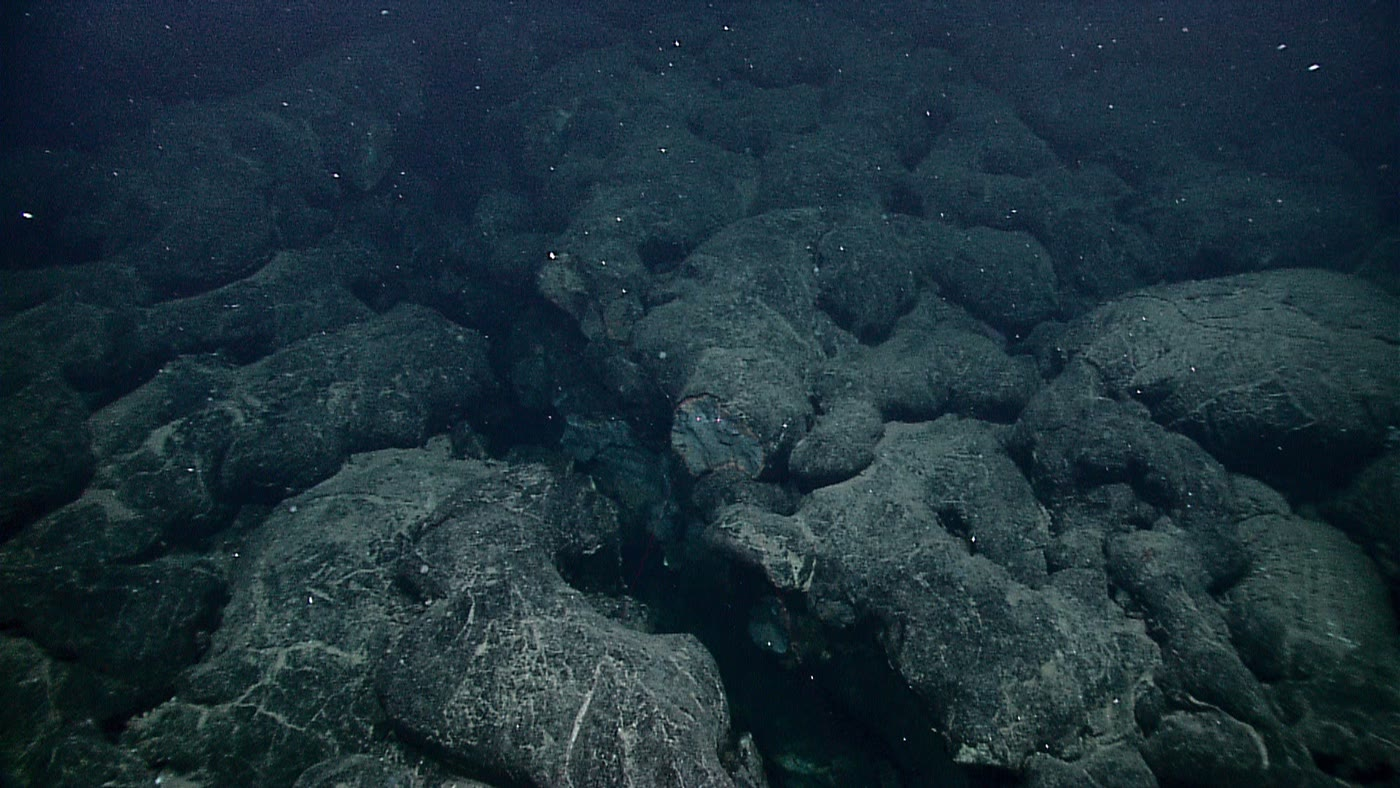
\includegraphics[width=0.6\linewidth]{images/book3/b1-pillow-lava.jpg}

\par\smallskip{\small \omterm{def:b1:rifts-ridges-margins:oceanic-crust}{Laves en coussins} sur le rift des Galápagos, coupées par une fissure
ouverte après leur solidification~: le sommet de la couche~2 de la \omterm{def:b1:rifts-ridges-margins:oceanic-crust}{croûte océanique} telle qu'elle
se forme. Chaque coussin est une langue de lave gelée de l'extérieur par l'eau
de mer. Photographie~: NOAA Okeanos Explorer Program, Galápagos Rift Expedition
2011, CC~BY~2.0 (Wikimedia Commons).}
\label{fig:b1:rifts-ridges-margins:pillows}
\end{omfigure}
% ledger: commons:pillow-expl6453

\begin{proposition}[Chaque dyke fend le précédent]\label{prop:b1:rifts-ridges-margins:dykes}
Supposons que chaque dyke d'un \omterm{def:b1:rifts-ridges-margins:oceanic-crust}{complexe filonien} soit injecté le long de l'axe
d'expansion, là où la \omterm{def:b1:layered-earth:layers}{croûte} est la plus chaude et la plus faible, et que la \omterm{def:b1:layered-earth:layers}{croûte} s'éloigne
de l'axe symétriquement. Alors la plupart des dykes sont trouvés fendus en deux, chaque
moitié avec une bordure figée seulement contre son voisin plus ancien.
\end{proposition}

\begin{proof}
Un dyke se fige contre la roche plus froide des deux côtés~: il a deux bordures
figées quand il se forme. Le dyke suivant monte là où la \omterm{def:b1:layered-earth:layers}{croûte} est la plus faible, le long de
l'axe, c'est-à-dire au milieu du précédent, encore la roche la plus chaude. Il
le fend en deux moitiés, que l'expansion emporte de part et d'autre~; chaque moitié garde la bordure figée
de son côté extérieur et a, du côté intérieur, le contact non refroidi
avec le nouveau dyke. Chaque dyke sauf le dernier est fendu de cette
façon.
\end{proof}

Les dykes avec une bordure figée d'un seul côté sont bien la règle dans les \omterm{def:b1:rifts-ridges-margins:oceanic-crust}{complexes filoniens}~:
la signature d'une \omterm{def:b1:layered-earth:layers}{croûte} construite, dyke après dyke, par
l'expansion.


\section{La loi profondeur--âge}\label{sec:b1:rifts-ridges-margins:depth-age}

Le plancher océanique est peu profond à la dorsale et profond loin d'elle. Comme le plancher est fait
à la dorsale et emporté, la distance à la dorsale est un âge, et la profondeur du
plancher dépend de son âge. La plaque se refroidit par le haut en vieillissant
(\cref{ch:b1:heat-budget})~; la roche froide est plus dense, et une colonne plus dense flotte
plus bas.

\begin{lemma}[Une intégrale de la fonction d'erreur]\label{lem:b1:rifts-ridges-margins:erfc}
Avec $\operatorname{erfc} u = 1 - \operatorname{erf} u =
\frac{2}{\sqrt\pi}\int_u^\infty e^{-s^2}\,\mathrm ds$,
\[
  \int_0^\infty \operatorname{erfc} u \,\mathrm du = \frac{1}{\sqrt\pi}.
\]
\end{lemma}

\begin{proof}
La dérivée de $\operatorname{erfc}$ est $-\frac{2}{\sqrt\pi}e^{-u^2}$.
En intégrant par parties sur $[0, X]$,
\[
  \int_0^X \operatorname{erfc} u\,\mathrm du
  = \bigl[u \operatorname{erfc} u\bigr]_0^X + \frac{2}{\sqrt\pi}\int_0^X u\,e^{-u^2}\,\mathrm du
  = X\operatorname{erfc} X + \frac{1}{\sqrt\pi}\bigl(1 - e^{-X^2}\bigr).
\]
Pour $X > 0$ et $s \ge X$, $e^{-s^2} \le (s/X)e^{-s^2}$, donc
$X\operatorname{erfc} X \le \frac{2}{\sqrt\pi}\int_X^\infty s\,e^{-s^2}\,\mathrm ds
= e^{-X^2}/\sqrt\pi$, qui tend vers 0. En faisant $X \to \infty$ on obtient le
résultat.
\end{proof}

\begin{theorem}[Loi profondeur--âge]\label{thm:b1:rifts-ridges-margins:depth-age}
Supposons que
\begin{enumerate}
  \item le \omterm{def:b1:layered-earth:layers}{manteau} quitte la dorsale à la température uniforme $T_m$, et la
        plaque océanique d'âge $t$ est un demi-espace refroidi depuis lors par sa
        surface, maintenue à $T_0$, avec la diffusivité thermique $\kappa$~;
  \item la masse volumique de la roche refroidie est $\rho_m\bigl(1 + \alpha(T_m -
        T)\bigr)$, avec $\rho_m$ la masse volumique du \omterm{def:b1:layered-earth:layers}{manteau} à $T_m$ et
        $\alpha$ son coefficient de dilatation thermique~;
  \item chaque colonne est en équilibre isostatique au-dessus d'une \omterm{def:b1:isostasy-gravity:isostasy}{profondeur de compensation}
        située sous la couche refroidie, et l'eau de mer a la masse volumique $\rho_w$.
\end{enumerate}
Alors la profondeur du fond marin d'âge $t$ est
\[
  d(t) = d_r + C\sqrt t, \qquad
  C = \frac{2}{\sqrt\pi}\,\frac{\rho_m\,\alpha\,(T_m - T_0)\sqrt\kappa}{\rho_m - \rho_w},
\]
où $d_r$ est la profondeur de l'axe de la dorsale. C'est la
\emph{loi profondeur--âge}\index{loi profondeur--age@loi profondeur--âge} du plancher océanique.
\end{theorem}

\begin{proof}
La température dans le demi-espace refroidi est
\[
  T(z, t) = T_0 + (T_m - T_0)\operatorname{erf}\frac{z}{2\sqrt{\kappa t}},
\]
avec $z$ la profondeur sous le fond marin~; cette solution de l'équation de la chaleur est
admise ici, comme au \cref{ch:b1:heat-budget}, et démontrée dans le volume de troisième
année. Comparons la colonne à la dorsale, faite d'eau jusqu'à $d_r$ et de
\omterm{def:b1:layered-earth:layers}{manteau} à $T_m$ en dessous, avec la colonne d'âge $t$, faite d'eau jusqu'à $d$ et
de la plaque refroidie en dessous, toutes deux jusqu'à la \omterm{def:b1:isostasy-gravity:isostasy}{profondeur de compensation} $D$. Leurs masses
par unité d'aire sont égales~:
\[
  \rho_w d_r + \rho_m (D - d_r) = \rho_w d + \int_0^{D-d}\rho_m\bigl(1 + \alpha(T_m - T)\bigr)\mathrm dz
  = \rho_w d + \rho_m (D - d) + \rho_m\alpha\int_0^{D-d}(T_m - T)\,\mathrm dz.
\]
D'où
\[
  (\rho_m - \rho_w)(d - d_r) = \rho_m\alpha\int_0^{D-d}(T_m - T)\,\mathrm dz.
\]
Puisque $T_m - T = (T_m - T_0)\operatorname{erfc}\bigl(z/2\sqrt{\kappa t}\bigr)$ est
négligeable sous la couche refroidie, l'intégrale peut être prise jusqu'à l'infini~; avec
$u = z/2\sqrt{\kappa t}$ et le \cref{lem:b1:rifts-ridges-margins:erfc},
\[
  \int_0^\infty (T_m - T)\,\mathrm dz = (T_m - T_0)\,2\sqrt{\kappa t}\int_0^\infty\operatorname{erfc}u\,\mathrm du
  = \frac{2}{\sqrt\pi}(T_m - T_0)\sqrt{\kappa t}.
\]
En divisant par $\rho_m - \rho_w$ on obtient $d - d_r = C\sqrt t$.
\end{proof}

L'eau compte~: quand la plaque s'enfonce, l'eau remplit l'espace au-dessus d'elle, et son
poids presse encore la plaque vers le bas. Le coefficient de dilatation effectif
$\alpha\rho_m/(\rho_m - \rho_w)$ est plus grand que $\alpha$ du facteur
$3300/2300 \approx 1.43$.

Avec $\alpha = \qty{3.2e-5}{K^{-1}}$, $T_m - T_0 = \qty{1350}{K}$,
$\kappa = \qty{e-6}{m^2.s^{-1}}$, $\rho_m = \qty{3300}{kg.m^{-3}}$ et
$\rho_w = \qty{1000}{kg.m^{-3}}$, et le temps compté en millions d'années
($\sqrt{\kappa\times\qty{1}{\Ma}} = \qty{5618}{m}$), le théorème donne
$C = \qty{393}{m.\Ma^{-1/2}}$. Les constantes ajustées par Parsons et Sclater sur
les profondeurs du Pacifique nord et de l'Atlantique nord, une fois les sédiments
retirés, en sont proches~: $d_r \approx \qty{2500}{m}$ et
$C \approx \qty{350}{m.\Ma^{-1/2}}$, de 0 à \qty{70}{\Ma}. Les valeurs de
$\alpha$ et $T_m$ utilisées ci-dessus sont celles de leur modèle de plaque pour le vieux plancher,
un \omterm{def:b1:layered-earth:layers}{manteau} à \qty{1350}{\degreeCelsius} et
$\alpha = \qty{3.2e-5}{\per\degreeCelsius}$, incertaines d'un cinquième et d'un tiers
respectivement, si bien que l'accord de 393 avec 350 est aussi bon qu'on pouvait
l'espérer.
% ledger: parsons:plate-model, ps77:depth-age

\begin{example}[Plancher océanique de 25 et de 100 millions d'années]\label{ex:b1:rifts-ridges-margins:depths}
Avec $d = 2500 + 350\sqrt t$ (mètres, $t$ en millions d'années), un plancher
de \qty{25}{\Ma} se trouve à $2500 + 350\times5 = \qty{4250}{m}$ et un plancher
de \qty{100}{\Ma} à $2500 + 350\times10 = \qty{6000}{m}$. Le plancher s'enfonce de
\qty{1750}{m} pendant ses 25 premiers millions d'années, et de seulement \qty{1750}{m} de plus pendant
les 75 suivants.
\end{example}
% ledger: parsons:plate-model

\begin{omfigure}
\begin{tikzpicture}
\begin{axis}[omrecord, omdepth, width=0.84\linewidth, height=6.6cm,
  xmin=0, xmax=13.6, ymin=2000, ymax=6800,
  xlabel={racine carrée de l'âge du plancher, $\sqrt t$ (\unit{\Ma^{1/2}})},
  ylabel={profondeur (\unit{m})},
  yticklabel style={/pgf/number format/set thousands separator={}},
  legend style={font=\scriptsize, at={(0.02,0.03)}, anchor=south west, draw=none, fill=white, fill opacity=0.85, text opacity=1},
  legend cell align=left]
% computed in figdata/bachelor-1/depth_age.py; ledger: data:etopo1, data:b2-seafloor-age, parsons:plate-model
\addplot[name path=lo, draw=none, forget plot] table[x expr=sqrt(\thisrow{t}), y=q1] {figdata/out/bachelor-1-depth_age-bins.dat};
\addplot[name path=hi, draw=none, forget plot] table[x expr=sqrt(\thisrow{t}), y=q3] {figdata/out/bachelor-1-depth_age-bins.dat};
\addplot[black!12] fill between[of=lo and hi];
\addlegendentry{moitié centrale des cellules}
\addplot[only marks, mark=*, mark size=1.1pt, black!70] table[x expr=sqrt(\thisrow{t}), y=median] {figdata/out/bachelor-1-depth_age-bins.dat};
\addlegendentry{profondeur médiane, classes d'âge de 2~Ma}
\addplot[very thick, omProp] table[x expr=sqrt(\thisrow{t}), y=halfspace] {figdata/out/bachelor-1-depth_age-models.dat};
\addlegendentry{demi-espace, $2500 + 350\sqrt t$}
\addplot[thick, omDef, densely dashed] table[x expr=sqrt(\thisrow{t}), y=plate] {figdata/out/bachelor-1-depth_age-models.dat};
\addlegendentry{modèle de plaque, $6400 - 3200\,e^{-t/62.8}$}
\draw[black!50, densely dotted] (axis cs:8.944,2000) -- (axis cs:8.944,6800);
\node[font=\scriptsize, anchor=north west, black!70] at (axis cs:8.944,2060) {\qty{80}{\Ma}};
\node[font=\scriptsize, anchor=north west, black!70] at (axis cs:4.472,2060) {\qty{20}{\Ma}};
\draw[black!50, densely dotted] (axis cs:4.472,2000) -- (axis cs:4.472,6800);
\end{axis}
\end{tikzpicture}

\par\smallskip{\small Profondeur du plancher océanique en fonction de la racine carrée de son
âge. Chaque point est la profondeur médiane des cellules d'un degré de l'océan mondial
dont le plancher tombe dans une classe d'âge de deux millions d'années (31\,538 cellules, plus profondes que
\qty{1000}{m})~; la bande grise contient la moitié centrale d'entre elles. La loi du demi-espace
est une droite sur ce graphique. Le jeune plancher la suit de près~; le plancher plus ancien
se trouve au-dessus, parce que les cellules portent leurs sédiments et comprennent des monts sous-marins
et des plateaux volcaniques, et parce que le vieux plancher cesse de s'enfoncer (en tirets~: le modèle
de plaque). Données~: ETOPO1 (NOAA) et âges du plancher océanique de Seton et
collab. (2020).}
\label{fig:b1:rifts-ridges-margins:depth-age}
\end{omfigure}

La figure teste le théorème sur tout l'océan. Jusqu'à environ
\qty{20}{\Ma} ($\sqrt t \approx 4.5$) les médianes se situent à une centaine de
mètres de la loi. Une droite ajustée aux médianes plus jeunes
que \qty{70}{\Ma} n'a qu'une pente de \qty{250}{m.\Ma^{-1/2}}~: les profondeurs mesurées
sont celles de la surface des sédiments, alors que la loi donne la profondeur du
sommet de la \omterm{def:b1:layered-earth:layers}{croûte}, et la couverture sédimentaire s'épaissit avec l'âge. Entre 60 et
\qty{80}{\Ma}, le plancher s'écarte de la loi en racine carrée même une fois ses
sédiments retirés~: il devient moins profond que la loi, et cesse de s'enfoncer.
Le modèle de plaque, une plaque épaisse de \qty{125}{km} dont la base est maintenue à la
température du \omterm{def:b1:layered-earth:layers}{manteau}, décrit cet aplatissement~: sa profondeur tend vers environ
\qty{6400}{m}, et son flux de chaleur vers une constante, comme si de la chaleur était apportée à la
base des vieilles plaques par le \omterm{def:b1:layered-earth:layers}{manteau} en convection. Ce modèle est étudié dans le
volume de troisième année~; dans ce livre la loi en racine carrée est utilisée jusqu'à \qty{80}{\Ma}.
% ledger: parsons:plate-model; fit and cell count from depth_age.py (values part)

\begin{method}[Dater le plancher océanique à partir de sa profondeur]\label{met:b1:rifts-ridges-margins:age-from-depth}
Pour estimer l'âge du plancher océanique là où ses anomalies magnétiques sont absentes ou
non cartographiées~:
\begin{enumerate}
  \item mesurer la profondeur du plancher et, à partir de profils sismiques,
        l'épaisseur de ses sédiments~; prendre la profondeur $d$ du sommet de la \omterm{def:b1:layered-earth:layers}{croûte},
        corrigée du poids des sédiments~;
  \item inverser la loi~: $t = \bigl((d - d_r)/C\bigr)^2$, avec $d_r$ et $C$ de
        l'océan concerné~;
  \item vérifier que le plancher est plus jeune qu'environ \qty{80}{\Ma}, et estimer
        l'incertitude~: une erreur $\delta d$ sur la profondeur donne
        $\delta t = 2t\,\delta d/(d - d_r)$.
\end{enumerate}
\end{method}

Pour un plancher à \qty{4600}{m}, $t = (2100/350)^2 = \qty{36}{\Ma}$, et une
incertitude de \qty{100}{m} sur la profondeur donne $2\times36\times100/2100 \approx
\qty{3.4}{\Ma}$ sur l'âge. Là où le plancher est moins profond que ne le prédit la loi sur
une vaste région, un bombement, la cause n'est pas l'âge mais la chaleur venue du dessous
(\cref{ch:b1:hotspots}).

La loi relie aussi l'océan au niveau de la mer. Une dorsale qui s'ouvre plus vite
emporte du plancher jeune et peu profond plus loin de son axe~; les bassins océaniques contiennent moins
d'eau, et la mer monte sur les continents. Sur des dizaines de millions d'années,
les variations de la vitesse d'expansion sont l'une des deux principales causes des variations du
niveau marin mondial, avec le volume de glace sur terre.

\section{Failles transformantes et zones de fracture}

Les dorsales ne sont pas des lignes continues~: elles sont découpées en segments décalés par des failles
qui leur sont perpendiculaires, selon la direction de l'expansion. Au-delà des décalages, les failles se prolongent en longues cicatrices
à travers le plancher océanique.

\begin{definition}[Faille transformante, zone de fracture]\label{def:b1:rifts-ridges-margins:transform}
Une \emph{faille transformante}\index{faille transformante} est une faille décrochante qui est
une limite de plaques et se termine sur d'autres limites de plaques~; une transformante
dorsale--dorsale relie les extrémités de deux segments de dorsale décalés. Une \emph{zone de
fracture}\index{zone de fracture} est le prolongement d'une faille transformante au-delà des
extrémités des segments de dorsale~: une vallée ou un ressaut linéaire à travers le plancher océanique
séparant des planchers d'âges différents qui appartiennent à une seule plaque.
\end{definition}

\begin{proposition}[Glissement sur une transformante dorsale--dorsale]\label{prop:b1:rifts-ridges-margins:transform}
Deux segments de dorsale s'ouvrant symétriquement à la demi-vitesse $u$, perpendiculairement
à eux-mêmes, sont décalés par une \omterm{def:b1:rifts-ridges-margins:transform}{faille transformante} de longueur $a$. Alors~:
\begin{enumerate}
  \item les deux côtés de la transformante glissent l'un contre l'autre à la vitesse totale
        $2u$, dans le sens opposé à celui que suggérerait le décalage si une
        dorsale droite unique avait été coupée et déplacée par la faille~;
  \item le long des \omterm{def:b1:rifts-ridges-margins:transform}{zones de fracture} les deux côtés ne se déplacent pas l'un par rapport à
        l'autre, et le plancher des deux côtés diffère d'âge de $a/u$~;
  \item la longueur de la transformante ne change pas avec le temps.
\end{enumerate}
\end{proposition}

\begin{proof}
Prenons l'axe $x$ le long de la transformante, vers l'est, et l'axe $y$
vers le nord, dans le repère de la dorsale. Soit le segment nord sur
$x = 0$, $y > 0$, et le segment sud sur $x = a$, $y < 0$ (le décalage est vers
l'est en allant vers le sud)~; la transformante est le segment $0 < x < a$ de $y = 0$. La
plaque ouest $W$ est à l'ouest des deux segments et se déplace à $-u$ selon $x$~; la
plaque est $E$ est à l'est des deux et se déplace à $+u$.

(1) Juste au nord de la transformante, pour $0 < x < a$, le plancher est à l'est du
segment nord~: il appartient à $E$ et se déplace vers l'est à $u$. Juste au sud, le
plancher est à l'ouest du segment sud~: il appartient à $W$ et se déplace vers l'ouest à
$u$. Le côté nord se déplace vers l'est à $2u$ par rapport au côté sud~: vu
de l'un ou l'autre côté, le côté opposé se déplace vers la droite, et le glissement est
dextre. Une dorsale droite coupée par la faille, sa partie sud
maintenant à l'est de sa partie nord, enregistrerait au contraire un déplacement
senestre.

(2) Pour $x > a$, les deux côtés sont à l'est de leurs segments et appartiennent à $E$~: ils
se déplacent ensemble. À la distance $x$ du segment nord, le plancher au nord de
la \omterm{def:b1:rifts-ridges-margins:transform}{zone de fracture} a l'âge $x/u$~; le plancher au sud est à $x - a$ du
segment sud et a l'âge $(x - a)/u$. La différence est $a/u$. Il en va de même
pour $x < 0$, où les deux côtés appartiennent à $W$.

(3) Les deux segments restent en $x = 0$ et $x = a$ dans le repère de la dorsale, puisque
chacun s'ouvre symétriquement~: la transformante garde la longueur $a$.
\end{proof}

J.\ Tuzo Wilson vit en 1965 que les décalages de dorsales ne peuvent se lire comme le
déplacement d'une dorsale droite plus ancienne, et prédit le sens du glissement
de la proposition~; les mécanismes au foyer des séismes sur les transformantes
l'ont confirmé. Les séismes se produisent le long de la transformante active, entre les extrémités de
dorsale~; les \omterm{def:b1:rifts-ridges-margins:transform}{zones de fracture} sont en général calmes. De part et d'autre d'une
\omterm{def:b1:rifts-ridges-margins:transform}{zone de fracture} le plancher des deux côtés a des âges différents, donc, par la
\omterm{thm:b1:rifts-ridges-margins:depth-age}{loi profondeur--âge}, des profondeurs différentes~: un ressaut qui s'estompe lentement avec la distance à
la dorsale. Dans l'Atlantique nord vers \ang{52}\,N, les deux
transformantes de Charlie--Gibbs décalent la dorsale médio-atlantique d'environ \qty{350}{km} au total.
% ledger: wilson:transform, data:pb2002 (offset summed over the transform steps in figdata/bachelor-1/ridge_budget.py)

\begin{omfigure}
\begin{tikzpicture}[x=0.95cm, y=0.95cm, font=\scriptsize]
\fill[omSea!10] (-5,-2.6) rectangle (8,2.6);
% isochrons (10 and 20 Myr), offset across the fracture zones
\foreach \x in {-4,-2,2,4} \draw[black!40] (\x,0) -- (\x,2.5);
\foreach \x in {-1,1,5,7} \draw[black!40] (\x,0) -- (\x,-2.5);
\node[black!55, anchor=south, fill=omSea!10, inner sep=1pt] at (2,2.0) {10};
\node[black!55, anchor=south, fill=omSea!10, inner sep=1pt] at (4,2.0) {20};
\node[black!55, anchor=south, fill=omSea!10, inner sep=1pt] at (-2,2.0) {10};
\node[black!55, anchor=south, fill=omSea!10, inner sep=1pt] at (-4,2.0) {20};
\node[black!55, anchor=north, fill=omSea!10, inner sep=1pt] at (5,-2.0) {10};
\node[black!55, anchor=north, fill=omSea!10, inner sep=1pt] at (7,-2.0) {20};
\node[black!55, anchor=north, fill=omSea!10, inner sep=1pt] at (1,-2.0) {10};
\node[black!55, anchor=north, fill=omSea!10, inner sep=1pt] at (-1,-2.0) {20};
% fracture zones and transform
\draw[black!60, thick, densely dashed] (-5,0) -- (0,0);
\draw[black!60, thick, densely dashed] (3,0) -- (8,0);
\draw[transform, line width=1.4pt] (0,0) -- (3,0);
% ridge segments
\draw[ridge, line width=1.1pt] (0,0) -- (0,2.6);
\draw[ridge, line width=1.1pt] (3,0) -- (3,-2.6);
\pic at (1.5,0) {dextral={90}};
\foreach \x in {0.4,0.75,2.25,2.6} \node[star, star points=5, star point ratio=2.2, fill=orange!90!black, draw=black, line width=0.2pt, inner sep=1.5pt] at (\x,0.0) {};
% plate motions
\draw[-{Stealth[length=4pt]}, very thick, black!70] (-2.8,1.1) -- (-3.9,1.1);
\draw[-{Stealth[length=4pt]}, very thick, black!70] (-0.2,-1.1) -- (-1.3,-1.1);
\draw[-{Stealth[length=4pt]}, very thick, black!70] (5.5,1.1) -- (6.6,1.1);
\draw[-{Stealth[length=4pt]}, very thick, black!70] (5.3,-1.1) -- (6.4,-1.1);
\node[font=\small] at (-3.3,1.55) {plaque $W$};
\node[font=\small] at (6.1,1.55) {plaque $E$};
\node[anchor=west, omRidge] at (0.1,2.25) {dorsale};
\node[anchor=east, omRidge] at (2.9,-2.25) {dorsale};
\node[anchor=north, align=center, fill=white, fill opacity=0.8, text opacity=1, inner sep=1pt] at (1.5,-0.35) {faille transformante\\(active, séismes)};
\node[anchor=south, fill=white, fill opacity=0.8, text opacity=1, inner sep=1pt] at (5.5,0.12) {zone de fracture (inactive)};
\node[anchor=north, fill=white, fill opacity=0.8, text opacity=1, inner sep=1pt] at (-2.5,-0.12) {zone de fracture (inactive)};
\node[anchor=south, black!70, fill=omSea!10, inner sep=1pt] at (6.2,0.55) {plus ancien, plus profond};
\node[anchor=north, black!70, fill=omSea!10, inner sep=1pt] at (6.0,-0.45) {plus jeune, moins profond};
\end{tikzpicture}

\par\smallskip{\small Une dorsale décalée par une \omterm{def:b1:rifts-ridges-margins:transform}{faille transformante}, en vue de dessus, nord
en haut. Les deux plaques s'écartent de chaque segment (flèches noires)~; le long de la
transformante (rouge) elles glissent l'une contre l'autre de façon dextre (demi-flèches),
bien que le décalage de la dorsale paraisse senestre. Les lignes grises sont des
isochrones, étiquetées en millions d'années~: de part et d'autre de chaque \omterm{def:b1:rifts-ridges-margins:transform}{zone de fracture} (en tirets)
des planchers d'âges différents, donc de profondeurs différentes, sont côte à côte, mais les deux
côtés se déplacent ensemble. Étoiles~: séismes, confinés à la transformante.}
\label{fig:b1:rifts-ridges-margins:transform}
\end{omfigure}

Les transformantes sont la troisième sorte de preuve des mouvements de plaques du
\cref{ch:b1:plate-kinematics}~: une transformante suit la vitesse relative des
deux plaques, donc elle se trouve sur un \omterm{def:b1:spherical-astronomy:spherical-triangle}{petit cercle} autour de leur \omterm{def:b1:plate-kinematics:euler-pole}{pôle d'Euler}, et les
\omterm{def:b1:spherical-astronomy:spherical-triangle}{grands cercles} tracés perpendiculairement à plusieurs transformantes se coupent au pôle.
Les \omterm{def:b1:rifts-ridges-margins:transform}{zones de fracture}, suivies à travers le plancher océanique, enregistrent la direction du mouvement
dans le passé, comme les anomalies magnétiques en enregistrent la vitesse.

\section{Exercices}

\begin{exercise}[$\star$]\label{exo:b1:rifts-ridges-margins:1}
En 2005 un segment du rift de l'Afar long de \qty{60}{km} s'est ouvert de
jusqu'à \qty{8}{m}, et \qty{2.5}{km^3} de magma ont été injectés. (a) Si le dyke avait
été épais de \qty{8}{m} sur tout le segment, quelle aurait été sa hauteur moyenne~?
(b) À la vitesse des plaques de \qty{18}{mm.an^{-1}}, combien d'années de mouvement
une ouverture de \qty{8}{m} représente-t-elle~?
% ledger: wright:afar, morvel:ar-nb
\end{exercise}

\begin{exercise}[$\star$]\label{exo:b1:rifts-ridges-margins:2}
Un \omterm{def:b1:rifts-ridges-margins:rift}{demi-graben} est bordé par une faille bordière de \omterm{def:b1:cross-sections:throw}{rejet vertical} \qty{3.0}{km} et de \omterm{def:b1:geological-maps:attitude}{pendage}
\ang{60}, et recoupé par une faille antithétique plus petite de \omterm{def:b1:cross-sections:throw}{rejet vertical} \qty{0.8}{km} et de \omterm{def:b1:geological-maps:attitude}{pendage}
\ang{70}. (a) Calculer le \omterm{def:b1:cross-sections:throw}{rejet horizontal} de chaque faille et l'extension de la coupe.
(b) La coupe est maintenant large de \qty{25}{km}~: quelle était sa largeur avant la fracturation~?
\end{exercise}

\begin{exercise}[$\star$]\label{exo:b1:rifts-ridges-margins:3}
Classer les dorsales suivantes avec les limites de la définition, d'après leurs \omterm{def:b1:plate-kinematics:spreading-rate}{vitesses
totales d'expansion} calculées avec des vecteurs de plaques~: dorsale de Gakkel
\qty{12}{mm.an^{-1}}~; centre de la mer Rouge \qty{15}{mm.an^{-1}}~; dorsale de Reykjanes
\qty{19}{mm.an^{-1}}~; dorsale de Carlsberg occidentale \qty{23}{mm.an^{-1}}~; Atlantique
sud à \ang{20}\,S \qty{33}{mm.an^{-1}}~; dorsale est-Pacifique à
\ang{20}\,S \qty{143}{mm.an^{-1}}. Lesquelles s'attend-on à voir avoir une
vallée axiale, et lesquelles un haut axial~?
% ledger: morvel:eu-na, morvel:redsea, morvel:in-sm, morvel:nb-sa, morvel:nz-pa (rates computed with euler_velocities.py)
\end{exercise}

\begin{exercise}[$\star$]\label{exo:b1:rifts-ridges-margins:4}
Environ \qty{3.0}{km^2} de nouveau plancher océanique sont faits chaque année, avec une \omterm{def:b1:layered-earth:layers}{croûte}
épaisse de \qty{7.1}{km}. (a) Quel volume de \omterm{def:b1:layered-earth:layers}{croûte} est fait chaque année~? (b) À ce
rythme, combien de temps faudrait-il pour faire les \qty{3.028e8}{km^2} du plancher
océanique~? Comparer à l'âge du plus vieux plancher océanique, environ
\qty{190}{\Ma}, et expliquer pourquoi les deux n'ont pas à concorder.
% ledger: data:pb2002 (ridge_budget.py), white:crust, dd10:split, data:b2-seafloor-age
\end{exercise}

\begin{exercise}[$\star\star$]\label{exo:b1:rifts-ridges-margins:5}
Avec $d = 2500 + 350\sqrt t$ (mètres, $t$ en millions d'années)~: (a) calculer
la profondeur d'un plancher de 4, 36 et 64 millions d'années~; (b) trouver l'âge d'un plancher
situé à \qty{4600}{m} et à \qty{5300}{m}~; (c) de combien le plancher
s'enfonce-t-il entre 4 et \qty{36}{\Ma}, et entre 36 et \qty{64}{\Ma}~?
\end{exercise}

\begin{exercise}[$\star\star$]\label{exo:b1:rifts-ridges-margins:6}
Calculer la constante $C$ de la \omterm{thm:b1:rifts-ridges-margins:depth-age}{loi profondeur--âge}
(\cref{thm:b1:rifts-ridges-margins:depth-age}) pour $\alpha =
\qty{3.2e-5}{K^{-1}}$, $\rho_m = \qty{3300}{kg.m^{-3}}$, $\rho_w =
\qty{1000}{kg.m^{-3}}$, $T_m - T_0 = \qty{1350}{K}$ et $\kappa =
\qty{e-6}{m^2.s^{-1}}$, en \unit{m.\Ma^{-1/2}}. Refaire le calcul pour un \omterm{def:b1:layered-earth:layers}{manteau}
plus froid de \qty{250}{K}. Quelle constante le plancher d'un océan plus froid suivrait-il~?
% ledger: parsons:plate-model
\end{exercise}

\begin{exercise}[$\star\star$]\label{exo:b1:rifts-ridges-margins:7}
Le modèle de plaque donne le flux de chaleur du plancher océanique sous la forme $q = 11.3/\sqrt t$,
en unités de \qty{e-6}{cal.cm^{-2}.s^{-1}}, avec $t$ en millions d'années.
(a) Convertir la constante en \unit{mW.m^{-2}.\Ma^{1/2}} ($\qty{1}{cal} =
\qty{4.184}{J}$) et la comparer aux \qty{490}{mW.m^{-2}.\Ma^{1/2}} du
\cref{ch:b1:heat-budget}. (b) Calculer $q$ à 1, 10 et \qty{150}{\Ma}. La loi
a été ajustée sur un plancher de jusqu'à \qty{120}{\Ma}, et le modèle de plaque fait
tendre le flux de chaleur du plancher plus vieux vers une constante~: la valeur à
\qty{150}{\Ma} est-elle alors trop élevée ou trop basse~?
% ledger: parsons:plate-model, dd10:young-ocean
\end{exercise}

\begin{exercise}[$\star\star$]\label{exo:b1:rifts-ridges-margins:8}
Une dorsale orientée nord--sud est coupée en deux segments~; en allant vers le sud le long de la
dorsale, l'axe saute de \qty{40}{km} vers l'\emph{ouest} à une \omterm{def:b1:rifts-ridges-margins:transform}{faille transformante}.
(a) Quel est le sens du glissement sur la transformante~? (b) Que semble montrer le décalage de
la dorsale~? (c) Où le long de la ligne de la transformante les
séismes se produisent-ils, et pourquoi pas au-delà~?
\end{exercise}

\begin{exercise}[$\star\star$]\label{exo:b1:rifts-ridges-margins:9}
Les \omterm{def:b1:rifts-ridges-margins:transform}{zones de fracture} de Charlie--Gibbs décalent la dorsale médio-atlantique de
\qty{350}{km} au total~; la \omterm{def:b1:plate-kinematics:spreading-rate}{vitesse totale d'expansion} y est de \qty{21.2}{mm.an^{-1}}.
Traiter le décalage comme une seule transformante. (a) Quelle est la différence d'âge
de part et d'autre de la \omterm{def:b1:rifts-ridges-margins:transform}{zone de fracture}~? (b) Avec $d = 2500 + 350\sqrt t$, calculer le
ressaut de profondeur à travers la \omterm{def:b1:rifts-ridges-margins:transform}{zone de fracture} à l'extrémité de la transformante, puis à \qty{100}{km}
et \qty{1000}{km} au-delà.
% ledger: data:pb2002 (ridge_budget.py), morvel:eu-na (rate at 52.5 N 31.5 W from euler_velocities.py)
\end{exercise}

\begin{exercise}[$\star\star\star$]\label{exo:b1:rifts-ridges-margins:10}
Un bassin océanique est fait à vitesse constante et contient du plancher de tout âge de 0
à $A$ en aires égales. (a) Montrer que sa profondeur moyenne est $d_r +
\frac23C\sqrt A$. (b) Avec $d_r = \qty{2500}{m}$ et
$C = \qty{350}{m.\Ma^{-1/2}}$, comparer $A = \qty{180}{\Ma}$ et
$A = \qty{120}{\Ma}$. (c) Si l'expansion du bassin s'accélère de sorte que son
plancher le plus ancien soit de \qty{120}{\Ma} au lieu de \qty{180}{\Ma}, de combien
le niveau de la mer monte-t-il, en négligeant l'inondation des continents mais en tenant compte de la
charge de l'eau supplémentaire sur le plancher, qui s'enfonce de $\rho_w/(\rho_m - \rho_w)$
fois la montée ($\rho_m = 3300$, $\rho_w = \qty{1000}{kg.m^{-3}}$)~?
\end{exercise}

\begin{exercise}[$\star\star\star$]\label{exo:b1:rifts-ridges-margins:11}
Dans le cadre de la \cref{prop:b1:rifts-ridges-margins:transform}, le ressaut de profondeur
à travers une \omterm{def:b1:rifts-ridges-margins:transform}{zone de fracture} à la distance $x > a$ du segment de dorsale le plus éloigné
est $\Delta d = C\bigl(\sqrt{x/u} - \sqrt{(x - a)/u}\bigr)$. (a) Montrer que, pour
$x \gg a$, $\Delta d \approx Ca/(2\sqrt{ux})$. (b) Avec
$C = \qty{350}{m.\Ma^{-1/2}}$, $a = \qty{350}{km}$ et
$u = \qty{10.6}{km.\Ma^{-1}}$, comparer les ressauts exact et approché à
$x = 450$, 1350 et \qty{3350}{km}. Quand l'approximation est-elle bonne à
\qty{10}{\percent} près~?
\end{exercise}

\begin{exercise}[$\star\star\star$]\label{exo:b1:rifts-ridges-margins:12}
Comparer la loi du demi-espace $d_1(t) = 2500 + 350\sqrt t$ avec la loi de plaque
$d_2(t) = 6400 - 3200\,e^{-t/62.8}$. (a) Calculer $d_2 - d_1$ à 10, 20, 30 et
\qty{40}{\Ma}. (b) Montrer que les deux lois sont égales à un âge compris entre 20 et
\qty{30}{\Ma} et le trouver à \qty{0.1}{\Ma} près par dichotomie. (c) Comparer leurs
pentes en ce point. Pourquoi peut-on raccorder les deux lois à cet âge sans cassure
visible~?
% ledger: parsons:plate-model
\end{exercise}

\section{Problème~: La naissance d'un océan}

\begin{problem}[{Problème du week-end --- un continent étiré par ses failles, un
jeune océan mesuré par ses bandes, et la profondeur de son plancher à mesure qu'il vieillit}]
\label{pb:b1:rifts-ridges-margins:1}
% values: calc/ch13.py (Part I rift section and Part II profile invented for the
% problem; real Euler vector, chron ages and depth--age constants)
% ledger: morvel:sm-an, morvel:nb-an, morvel:ar-nb, morvel:redsea, morvel:outward, iodp:gpts2004, heine:sam-saf, parsons:plate-model, wright:afar
Prendre $R = \qty{6371}{km}$. Un océan naît en trois étapes, chacune visible aujourd'hui en un
lieu différent~: un \omterm{def:b1:rifts-ridges-margins:rift}{rift continental}, un jeune océan, un vieil océan.

\medskip
\noindent\textbf{Partie I --- Un rift étiré par ses failles.} Une coupe à travers
un rift orienté \ang{020} recoupe six failles normales dont les rejets verticaux et les \omterm{def:b1:geological-maps:attitude}{pendages} ont été
mesurés sur des profils sismiques~:
\begin{center}
\small
\begin{tabular}{lcccccc}
\hline
faille & F1 & F2 & F3 & F4 & F5 & F6\\
\omterm{def:b1:cross-sections:throw}{rejet vertical} (\unit{m}) & 600 & 1100 & 2400 & 350 & 800 & 1500\\
\omterm{def:b1:geological-maps:attitude}{pendage} & \ang{60} & \ang{55} & \ang{50} & \ang{65} & \ang{60} & \ang{52}\\
\hline
\end{tabular}
\end{center}
Les failles recoupent des laves datées de \qty{3.2}{Ma}, et le rift est maintenant large de \qty{60}{km}.
\begin{enumerate}
  \item Calculer le \omterm{def:b1:cross-sections:throw}{rejet horizontal} de chaque faille. Laquelle est la faille bordière~?
  \item Calculer l'extension de la coupe, et la largeur du rift avant
        la fracturation.
  \item Les deux plaques s'écartent à \qty{6.0}{mm.an^{-1}} vers \ang{105}.
        Calculer la composante de ce mouvement perpendiculaire au rift.
  \item Combien de temps les plaques mettraient-elles à produire l'extension de la question 2~?
  \item De combien les plaques se sont-elles écartées depuis l'émission des laves~?
        Quelle fraction en portent les failles~?
  \item Proposer où est passé le reste de l'extension. Si elle était reprise
        par des dykes comme celui de l'Afar en 2005, larges de \qty{8}{m}, combien en
        faudrait-il, et à quelle fréquence~?
\end{enumerate}

\medskip
\noindent\textbf{Partie II --- Un jeune océan mesuré par ses bandes.} Un
profil magnétique à travers l'axe du centre de la mer Rouge, à
\ang{18.0}\,N, \ang{40.0}\,E, mené selon la direction de l'expansion. Le bord
jeune du chron C2An (\qty{2.581}{Ma}) se trouve à \qty{21.0}{km} au nord-est de
l'axe et à \qty{20.2}{km} au sud-ouest~; le bord ancien du chron C3n
(\qty{5.235}{Ma}) à \qty{41.0}{km} et \qty{40.2}{km}. Les bords des
anomalies sont déplacés vers l'extérieur de l'axe de \qty{2.2}{km} au total, en
moyenne, sur les deux flancs.
\begin{enumerate}[resume]
  \item Calculer la \omterm{def:b1:plate-kinematics:spreading-rate}{vitesse totale d'expansion} pour chaque chron, sans correction.
  \item Corriger chaque vitesse du déplacement vers l'extérieur. Les deux concordent-elles~?
  \item Montrer que la vitesse calculée à partir de la distance entre les deux chrons sur
        chaque flanc ne demande aucune correction, et la calculer.
  \item Calculer les demi-vitesses sur chaque flanc à partir des distances entre les deux
        chrons. L'expansion est-elle symétrique~?
  \item Le \omterm{def:b1:plate-kinematics:euler-pole}{pôle d'Euler} de l'Arabie par rapport à la Nubie est à \ang{30.9}\,N,
        \ang{23.6}\,E, avec la vitesse \qty{0.403}{\degree\per\Ma}. Calculer la
        distance angulaire du pôle au profil, et la \omterm{def:b1:plate-kinematics:spreading-rate}{vitesse totale d'expansion} que
        le vecteur des plaques y prédit.
  \item Dans le nord de la mer Rouge, à \ang{26.0}\,N, \ang{35.0}\,E, calculer la
        distance angulaire au pôle et la vitesse prédite.
  \item Comparer ces vitesses à celles mesurées, 15 et
        \qty{9}{mm.an^{-1}}. Pourquoi la mer Rouge s'ouvre-t-elle plus vite au sud~?
\end{enumerate}

\medskip
\noindent\textbf{Partie III --- Vers un Atlantique.}
\begin{enumerate}[resume]
  \item Quelle est la largeur du plancher océanique fait dans le centre de la mer Rouge depuis le
        bord ancien de C3n, à la vitesse de la question 9~?
  \item L'Atlantique sud s'est ouvert d'environ \qty{5000}{km} à Recife en
        \qty{120.6}{\Ma} (\cref{ch:b1:plate-kinematics}). Calculer sa vitesse
        moyenne d'ouverture.
  \item À la vitesse actuelle du centre de la mer Rouge, combien de temps une ouverture
        de \qty{5000}{km} prendrait-elle~? Et à la vitesse du nord de la mer Rouge~?
  \item La mer Rouge s'ouvre autour d'un pôle proche d'elle. Qu'est-ce que cela implique pour
        sa forme à mesure qu'elle s'élargit, et pour le temps dont la partie nord a besoin pour
        atteindre la largeur qu'a maintenant la partie centrale~?
  \item De quel type de dorsale s'agit-il pour l'axe de la mer Rouge, et quelle forme d'axe
        attend-on~?
\end{enumerate}

\medskip
\noindent\textbf{Partie IV --- Le plancher s'enfonce.} Utiliser $d = 2500 + 350\sqrt t$
(mètres, $t$ en millions d'années) et, pour comparaison, la loi de plaque
$6400 - 3200\,e^{-t/62.8}$.
\begin{enumerate}[resume]
  \item Calculer la profondeur du nouveau plancher aux âges de 1, 10 et
        \qty{40}{\Ma}.
  \item À quel âge le plancher atteint-il \qty{4000}{m}~?
  \item Le plancher voisin de chaque \omterm{def:b1:rifts-ridges-margins:passive-margin}{marge passive} a l'âge de l'océan. De combien
        s'enfonce-t-il pendant les \qty{10}{\Ma} qui suivent la rupture, et entre
        70 et \qty{80}{\Ma}~?
  \item À quelle vitesse, en mètres par million d'années, ce plancher s'enfonce-t-il quand
        l'océan a \qty{80}{\Ma}~?
  \item Quel flux de chaleur le plancher de la question 22 perd-il alors, avec
        $q = 490/\sqrt t$ en \unit{mW.m^{-2}}~?
  \item Calculer la profondeur d'un plancher de \qty{80}{\Ma} avec chacune des deux
        lois, et leur différence. Pourquoi peut-on comparer les deux à cet âge~?
  \item Au dixième de kilomètre près, à quelle profondeur la loi en racine carrée
        place-t-elle le fond marin du nouvel océan quand il a 80 millions d'années~?
\end{enumerate}
\end{problem}
